\chapter{Company Profile: FlowGenX AI}
\label{ch:company}

This chapter introduces \textbf{FlowGenX AI} as an organisation:
its products, its agentic platform architecture, the technologies
that power it, the use cases it targets, and the working environment
it offers its employees and interns. The contents of this chapter
are drawn from FlowGenX AI's public website
(\texttt{https://www.flowgenx.ai/}), the internal repositories I
worked on during the internship, and direct conversations with the
engineering leadership.

\section{Company Overview}
\textbf{FlowGenX AI} is a software development company headquartered
in \textbf{San Francisco, California} that builds a next-generation
\emph{Agentic Integration Platform}. The platform allows enterprises
to design, orchestrate, and deploy AI agents and workflows from a
single, no-/low-code interface --- bringing together multi-agent
orchestration, native protocol-level integration with hundreds of
external services, a vector-powered knowledge base, and enterprise-grade
security and governance into one coherent product.

The company describes itself with the tagline
\emph{``Build Agentic Workflows. Automate Any Process, Integrate Any
App''} and positions its product as
\emph{``one platform to design, orchestrate, and deploy AI agents and
workflows --- from idea to production in minutes''}. In the broader
software market, the platform sits at the intersection of two
historically separate categories: \emph{integration platform as a
service} (iPaaS), which has historically been served by tools such as
Zapier, Make, n8n, and Workato; and the newer category of agentic AI
orchestration frameworks. FlowGenX AI's positioning is to unify
these two worlds: every integration becomes an intelligent tool that
agents can discover, reason about, and use.

% TODO (CEO confirmation): founding year, employee count globally,
% number of engineers based in Bangladesh, registered entity status
% in Bangladesh, funding stage. Placeholders below until confirmed.
At the time of writing, FlowGenX AI operates as a globally distributed
engineering team with team members in the United States and Bangladesh,
collaborating remotely through Google Chat and Google Meet. The
specific employee count, founding year, and Bangladesh entity status
will be incorporated into the final version of this report following
direct confirmation from the leadership team.

\section{Vision}
The company's vision, taken verbatim from its \emph{About} page, is:

\begin{quote}
``FlowGenX AI envisions a world where enterprise integration is
transformed through intelligent agentic orchestration. We break down
data silos, automate complex workflows, and enable seamless
integration between legacy systems and modern cloud platforms --- all
through our intuitive platform that puts the power of AI-driven
integration into the hands of both technical and non-technical
users.''
\end{quote}

This vision shapes everything about how the platform is built. Rather
than treating integration as a developer-only activity (the way
classical iPaaS tools do) or treating agentic AI as a research toy
(the way many open-source agent frameworks do), FlowGenX AI
deliberately blurs the line between the two. Workflows are first-class
citizens; so are agents; and connectors are the substrate through
which both interact with the rest of the world.

\section{What FlowGenX AI Does}
At a high level, FlowGenX AI helps enterprises do three things:

\begin{enumerate}[leftmargin=*]
    \item \textbf{Connect any system to any other system.} Through a
    catalogue of more than two hundred natively built connectors plus
    the ability to import any external API and auto-convert it into a
    Model Context Protocol (MCP) tool, the platform can talk to
    databases, cloud storage, SaaS applications, AI/LLM providers,
    helpdesks, CRMs, ERPs, and almost any other system an enterprise
    runs.

    \item \textbf{Compose those systems into intelligent workflows.}
    A visual, drag-and-drop workflow builder lets technical and
    non-technical users alike compose multi-step processes that move
    data, transform it, apply privacy policies, branch on conditions,
    iterate over collections, and call external services.

    \item \textbf{Add agentic intelligence on top of those workflows.}
    Multi-agent orchestration patterns (ReAct, Supervisor, Swarm, and
    Deep agent patterns) coordinate multiple AI agents that reason
    about the next step, distribute tasks among themselves, and
    collaborate in real time, all while remaining inside the same
    governed control plane as the deterministic workflow steps.
\end{enumerate}

This is captured in the company's promise of being a
\emph{``Complete Agentic Stack''}: agent orchestration, MCP-native
integrations, A2A communication, vector-powered knowledge base, and a
no-code workflow builder, all governed by a single control plane.

\section{The FlowGenX Platform}
The platform is organised around six functional pillars. Together they
form what FlowGenX calls the \emph{Complete Agentic Stack}.

\subsection{Multi-Agent Orchestration (Agent Fabric)}
A first-class agentic runtime that supports the most widely used
multi-agent design patterns out of the box --- including \textbf{ReAct},
\textbf{Supervisor}, \textbf{Swarm}, and \textbf{Deep} agent patterns.
Multiple agents can reason about the next step, distribute tasks
between themselves, and collaborate in real time. Agent execution is
observable, governable, and supports human-in-the-loop approval gates
at any step.

\subsection{Agentic Integration Engine (Integration Studio)}
The integration substrate of the platform. It exposes more than
\textbf{200 managed connectors} for databases, cloud storage,
software-as-a-service applications, and AI providers. In addition,
arbitrary external APIs can be imported and \emph{automatically
converted into MCP tools} that any agent can discover and call. This
is the layer my own work --- the
\texttt{runtime\_connectivity} project --- sits inside.

\subsection{Workflow Development}
A visual, drag-and-drop workflow builder where users compose
multi-step processes graphically. Workflows can be triggered by
events, run as batch jobs, or invoked on demand. They support inline
data transformation, privacy policies, conditional branching,
iteration, and full traceability across every step. Figure
\ref{fig:workflow-editor} shows the workflow editor.

\begin{figure}[H]
    \centering
    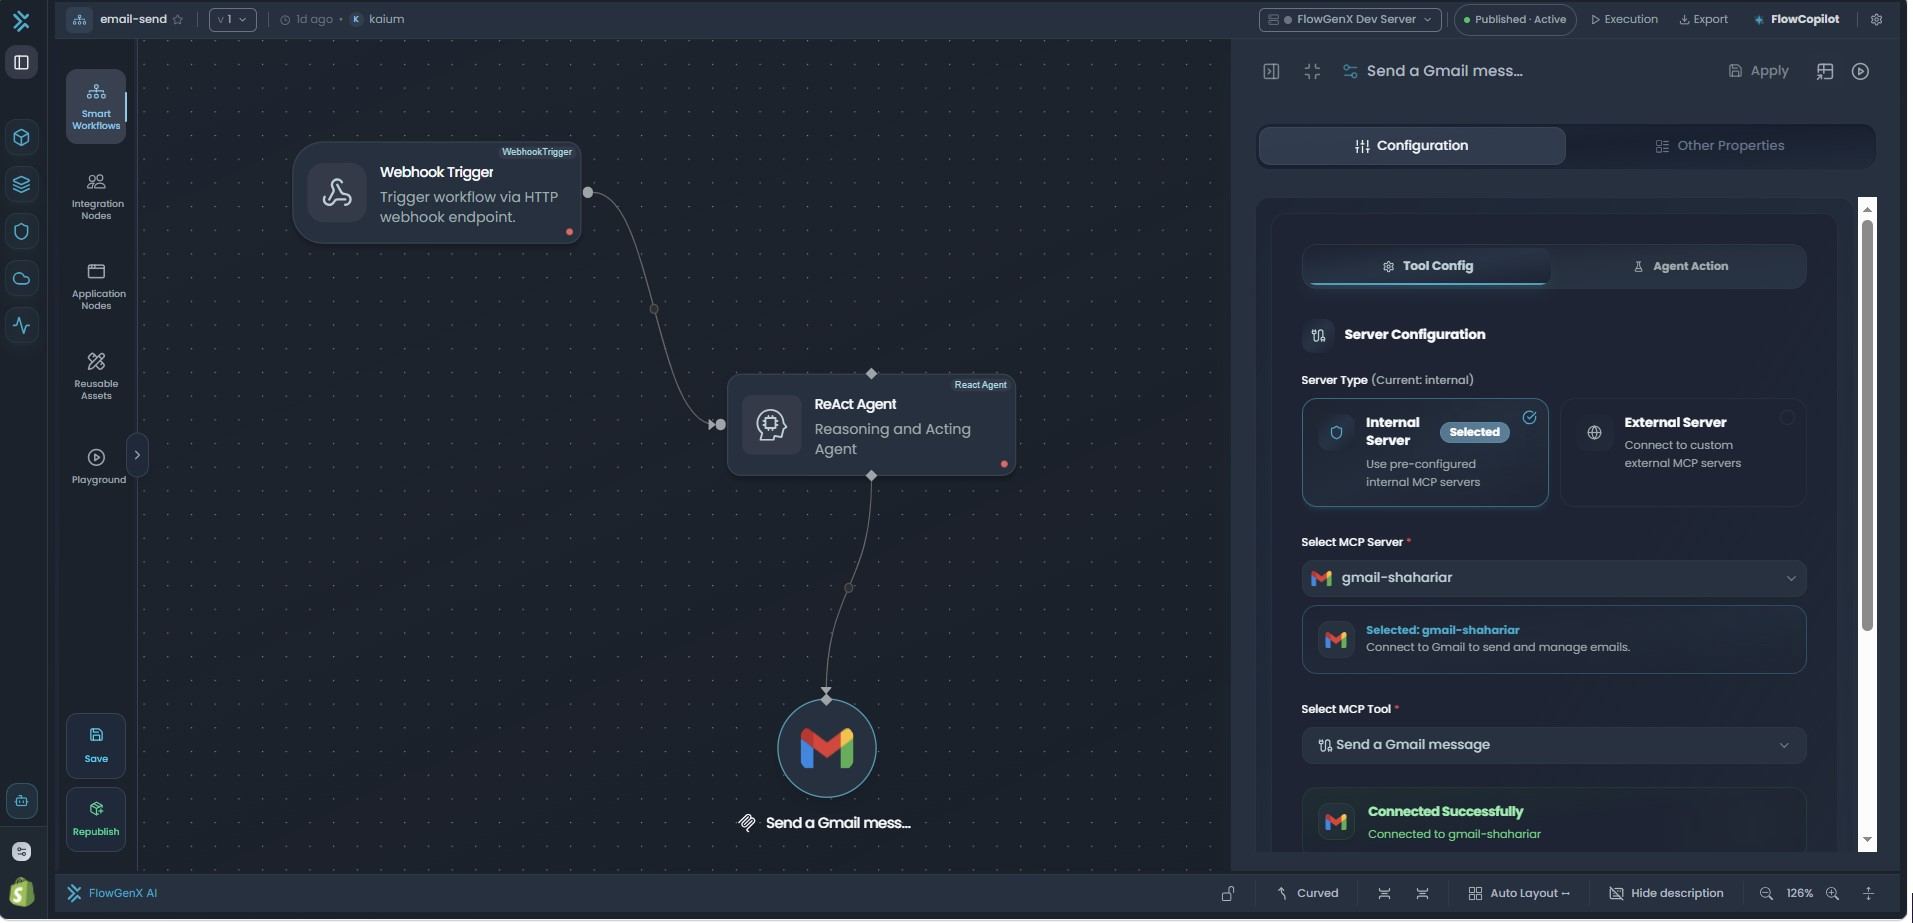
\includegraphics[width=0.95\textwidth]{figures/screenshots/workflow_editor.jpg}
    \caption{The FlowGenX AI visual workflow editor.}
    \label{fig:workflow-editor}
\end{figure}

\subsection{Intelligent Knowledge Base}
A vector-powered Retrieval-Augmented Generation (RAG) layer with
document ingestion, semantic search, and source citation. It
provides agents with grounded enterprise context so that answers
remain anchored in real source material rather than hallucinated.

\subsection{Work AI}
A suite of higher-level AI capabilities that sit on top of the agent
fabric and the workflow engine, intended to give end users a
copilot-style experience for everyday automation tasks.

\subsection{Security \& Governance (Agent Gateway)}
Enterprise-grade authentication, authorisation, and rate limiting for
every API, MCP tool, and agent. Provides full audit trails,
field-level encryption, and consumer access controls. Agents act
autonomously by default but always under the constraints set by the
governance layer; human-in-the-loop approval gates can be inserted
wherever judgement is required.

\section{Use Cases and Target Industries}
FlowGenX AI's public use-case catalogue covers eleven distinct
real-world scenarios across seven enterprise functions. Table
\ref{tab:flowgenx-usecases} summarises them.

\begin{table}[H]
\centering
\renewcommand{\arraystretch}{1.25}
\begin{tabularx}{\textwidth}{l l X}
\toprule
\textbf{Function} & \textbf{Use Case} & \textbf{What it does} \\
\midrule
Operations & Document Intelligence    & Extracts and reconciles data from PDFs, Excel, Word, and images, and pushes it into ERPs and CRMs. \\
Operations & Supply Chain Operations  & Monitors inventory, flags disruptions, and coordinates with suppliers autonomously. \\
IT         & IT Support Desk          & Resolves employee requests by triaging, routing, and closing tickets without human intervention. \\
IT         & IT Ticket Triage         & Classifies, prioritises, and assigns tickets in real time based on context and team capacity. \\
Sales      & CRM Enrichment           & Continuously researches and enriches contacts and accounts from the public web, SEC filings, and business databases. \\
Sales      & RFP Drafting             & Researches requirements and drafts complete RFP responses in minutes rather than days. \\
Compliance & Compliance Monitoring    & Monitors regulatory changes and surfaces internal-policy risks before they become violations. \\
Finance    & Financial Reporting      & Aggregates, reconciles, and formats board-ready financial reports on a recurring schedule. \\
HR         & HR Onboarding Automation & Provisions accounts, sends welcome materials, and guides new hires through their first day. \\
Marketing  & Email Campaign Operations& Segments audiences, personalises content, and tracks performance across multi-step campaigns. \\
Capability & Web App Automation       & Drives real browsers through enterprise web apps using structured DOM perception. \\
\bottomrule
\end{tabularx}
\caption{FlowGenX AI's published use cases across seven enterprise functions.}
\label{tab:flowgenx-usecases}
\end{table}

The breadth of these use cases reflects the platform's positioning:
the same underlying primitives (agents, workflows, connectors,
knowledge base) can be assembled to solve very different business
problems across operations, IT, sales, compliance, finance, HR, and
marketing.

\section{Tools and Technologies Utilised by FlowGenX AI}
FlowGenX AI has deliberately chosen a modern, polyglot, cloud-native
technology stack. The choices are visible in the codebases I worked
on directly.

\subsection{Programming Languages}
\begin{itemize}[leftmargin=*]
    \item \textbf{Backend:} Python 3.11+, used across the connectivity
    framework, the workflow APIs, and the reusable component library.
    \item \textbf{Frontend:} TypeScript and JavaScript, on top of
    React and Next.js.
    \item \textbf{Configuration and data exchange:} JSON, YAML, and
    OpenAPI 3.0 specifications.
    \item \textbf{Database queries:} SQL across PostgreSQL and
    multiple other relational engines (MySQL, MSSQL, Snowflake,
    Azure SQL, etc.).
\end{itemize}

\subsection{Backend Frameworks and Libraries}
\begin{itemize}[leftmargin=*]
    \item \textbf{API framework:} \emph{FastAPI} for the runtime APIs.
    \item \textbf{Workflow engine:} \emph{Apache Airflow} for
    pipeline scheduling, orchestration, and DAG-style execution of
    workflows.
    \item \textbf{Data validation and schema modelling:}
    \emph{Pydantic} (used pervasively for connection parameters,
    component schemas, and request/response models).
    \item \textbf{Data manipulation:} \emph{pandas} for in-memory
    DataFrame transformations.
    \item \textbf{Templating:} \emph{Jinja2} for dynamic, runtime-
    parameterised configuration of components.
    \item \textbf{HTTP and async I/O:} \emph{requests}, \emph{httpx},
    and \emph{asyncio}.
    \item \textbf{Cloud SDKs:} \emph{boto3} (AWS), the official Azure
    SDK for Python, and Google Cloud client libraries.
\end{itemize}

\subsection{Frontend Frameworks and Libraries}
\begin{itemize}[leftmargin=*]
    \item \textbf{Framework:} \emph{Next.js} on top of \emph{React}
    powers the FlowGenX web application (the \texttt{flowgenx-nextjs-V2}
    repository).
    \item \textbf{Runtime:} Node.js.
    \item \textbf{Editor experience:} The Monaco editor is integrated
    for in-browser code and expression editing.
\end{itemize}

\subsection{Databases and Search Technologies}
The platform supports a wide variety of data backends through the
connectivity framework I worked on.

\begin{itemize}[leftmargin=*]
    \item \textbf{Relational:} PostgreSQL (also the platform's own
    metadata store), MySQL, Microsoft SQL Server, Azure SQL Server,
    AWS RDS PostgreSQL and MySQL, Snowflake.
    \item \textbf{Document and NoSQL:} MongoDB.
    \item \textbf{Search:} Elasticsearch, Typesense.
    \item \textbf{Vector databases:} Pinecone, Weaviate, Milvus
    (used both as connectors and to support the platform's own
    Knowledge Base feature).
\end{itemize}

\subsection{Cloud Infrastructure and DevOps}
\begin{itemize}[leftmargin=*]
    \item \textbf{Cloud providers:} Amazon Web Services (S3, RDS,
    Textract, Rekognition, EC2), Microsoft Azure (Blob Storage,
    Data Lake, SQL Server), Google Cloud Platform.
    \item \textbf{Containerisation and orchestration:} Docker for
    containerisation, Kubernetes for orchestration, and Helm for
    Kubernetes packaging.
    \item \textbf{Infrastructure as Code:} Terraform.
    \item \textbf{API documentation:} OpenAPI / Swagger,
    auto-generated from connector source code.
\end{itemize}

\subsection{AI / LLM Providers and Generative AI Stack}
A direct implication of being an agentic platform is first-class
support for many AI providers. Through native connectors, the platform
integrates with:

\begin{itemize}[leftmargin=*]
    \item OpenAI (assistants, models, threads).
    \item Anthropic (messages, batch, files, models, and the new
    Skills API).
    \item Google Gemini and Vertex AI.
    \item xAI, Groq, DeepSeek, Perplexity AI.
    \item AWS-native AI services: Textract for document analysis and
    Rekognition for vision.
    \item Search and research providers: Tavily, Exa, SerpAPI.
\end{itemize}

On top of these providers, the platform implements multi-agent
orchestration patterns (ReAct, Supervisor, Swarm, and Deep), the
Model Context Protocol (MCP) for tool exposure, and an
Agent-to-Agent (A2A) protocol for inter-agent communication.

\subsection{Authentication and Identity}
The connectivity framework supports the full spectrum of authentication
patterns used by modern APIs:

\begin{itemize}[leftmargin=*]
    \item OAuth 2.0 with refresh-token flows.
    \item API Key and Bearer Token authentication.
    \item HTTP Basic Authentication.
    \item AWS IAM credentials and signed-request flows.
\end{itemize}

\subsection{Engineering Tooling}
\begin{itemize}[leftmargin=*]
    \item \textbf{Version control:} Git, hosted on GitHub.
    \item \textbf{Python package management:} \emph{uv}.
    \item \textbf{Code formatting:} Black (with a 79-character line
    length).
    \item \textbf{Import sorting:} isort, configured with the
    \emph{black} profile.
    \item \textbf{Linting:} Ruff, with selected rule sets.
    \item \textbf{Pre-commit hooks:} enforce all of the above
    automatically before each commit.
    \item \textbf{Project management:} ClickUp.
    \item \textbf{Communication:} Google Chat and Google Meet.
\end{itemize}

\section{Internal Architecture (At a High Level)}
The platform is organised across four primary internal repositories,
each with a clear single responsibility:

\begin{itemize}[leftmargin=*]
    \item \texttt{flowgenx-nextjs-V2} --- the customer-facing web
    application built on Next.js and React. This is what users
    interact with when they design workflows, configure connectors,
    or chat with their agents.

    \item \texttt{runtime\_apis} --- the FastAPI service that exposes
    workflow execution and component management endpoints, backed by
    Apache Airflow as the underlying workflow engine and PostgreSQL
    for state. The repository describes itself as
    \emph{``a flexible and scalable data pipeline workflow platform
    that combines Apache Airflow's workflow management capabilities
    with FastAPI's modern API development features''}.

    \item \texttt{runtime\_components} --- a reusable Python library
    of pipeline components used by the workflow engine. It currently
    ships ten or more pre-built components, including
    \texttt{IngestionComponent}, \texttt{FilterComponent},
    \texttt{DataMappingComponent}, \texttt{DataPrivacyComponent}
    (with built-in masking and anonymisation for credit-card numbers,
    SSNs, addresses, email, and other PII),
    \texttt{WriteComponent}, \texttt{JoinerComponent},
    \texttt{HTTPNodeComponent}, \texttt{ForeachComponent},
    \texttt{SwitchComponent}, and \texttt{SensorComponent}. All
    components are configured through Pydantic-validated schemas and
    can be parameterised at runtime through Jinja2 expressions.

    \item \texttt{runtime\_connectivity} --- the unified connectivity
    framework I contributed to, which exposes external services
    through a single standardised interface. This repository is the
    subject of Chapter~4.
\end{itemize}

\section{Office Environment and Working Style}
% TODO (CEO confirmation): Bangladesh entity status, exact team sizes
FlowGenX AI operates as a remote-first organisation with engineers
based in the United States and Bangladesh. My own internship was a
fully remote engagement from Dhaka, working on my personal laptop.

\begin{itemize}[leftmargin=*]
    \item \textbf{Communication tools.} The team uses Google Chat for
    asynchronous messaging and Google Meet for synchronous discussions
    and daily standups. Microsoft Teams was used previously and was
    migrated away from during my tenure.

    \item \textbf{Project management.} Work is tracked on
    \emph{ClickUp} boards, with each connector and feature represented
    as a card with status, assignee, and links to the relevant pull
    request.

    \item \textbf{Working hours.} I generally worked from
    approximately 9:00\,a.m. to 5:00\,p.m. Bangladesh Standard Time
    (UTC+6), with flexibility to shift hours when needed to overlap
    with the United States team for synchronous meetings.

    \item \textbf{Cadence.} The team operates with daily asynchronous
    updates and synchronous reviews when needed. Sprint cadence and
    formal release-cycle naming are confirmed in Chapter~3.
\end{itemize}

\section{Company Culture}
The cultural traits I directly experienced over five and a half
months at FlowGenX AI are:

\begin{itemize}[leftmargin=*]
    \item \textbf{Ownership and autonomy.} From my first connector
    onwards, I was trusted to design and ship features end-to-end ---
    research the third-party API, design the connection-parameter
    schema, implement the manager class and methods, write integration
    tests, generate the metadata, open the pull request, address
    review feedback, and merge.

    \item \textbf{Mentorship over micromanagement.} My supervisor
    Mr.~Abrar Bin Rofique reviewed every pull request thoroughly and
    explained the \emph{why} behind every suggestion, but never
    micromanaged the \emph{how}. The same was true of my team lead.

    \item \textbf{Quality through automation.} Pre-commit hooks
    running Black, isort, and Ruff catch style issues before they
    reach review. Pull requests cannot be merged without passing
    these checks. The result is a codebase that is genuinely uniform
    across many contributors.

    \item \textbf{Innovation and curiosity.} Engineers are
    encouraged to learn and to bring back new patterns. During my
    internship I was given room to explore the Model Context Protocol,
    the Agent-to-Agent protocol, and the workflow engine's internals
    --- all beyond the strict scope of my connector work.

    \item \textbf{Continuous learning.} The company maintains an
    extensive blog (\texttt{https://blog.flowgenx.ai/}) and developer
    documentation (\texttt{https://docs.flowgenx.ai/}) that engineers
    are encouraged to read and contribute to.

    \item \textbf{Impact over titles.} As stated in my offer letter,
    the company values \emph{``a culture of innovation, ownership,
    and continuous learning that values impact over titles.''} As
    an intern I felt this concretely: my work on the
    \texttt{runtime\_connectivity} project ships to the same end users
    as work from the most senior engineers on the team.
\end{itemize}
